\documentclass[12pt,a4paper]{article}
\usepackage{times}
\usepackage{durhampaper}
\usepackage{harvard}
\usepackage{float}
\usepackage{graphicx}
\citationmode{abbr}
\bibliographystyle{agsm}
\usepackage[dvipsnames]{xcolor}
\title{Image Processing using JavaScript and Web Assembly}
\author{} % leave; your name goes into \student{}
\student{Sam Robbins}
\supervisor{Tom Friedetzky}
\degree{BSc Computer Science}

\date{}

\begin{document}

\maketitle

\begin{abstract}
    \subsection{Context/Background}
    Web Assembly is a relatively new method for computation on the web, allowing for the use of a much wider range of languages. This is being used in high intensity contexts to improve computation time.

    \subsection{Aims}

    To determine in which cases implementing algorithms in web assembly is the right choice to make

    \subsection{Method}

    Implement a range of image processing algorithms in both JavaScript and Web Assembly and measure using a variety of metrics.

    \subsection{Results}

    \subsection{Conclusions}
\end{abstract}

\begin{keywords}
    Put a few keywords here.
\end{keywords}

\newpage

\section{Introduction}

Image processing is a widely used technique for a range of problems. In most modern cameras there will be some aspect of image processing at the time of capture, whether it is enhancements to the image or just the formatting to a file type, such as JPEG. After capture there is often additional image processing, be it applying filters or compression for upload online. Sophisticated image processing techniques don't just have benefit for the sharing of photos, but are also used medically, such as for processing CT images \cite{zhang2017applications}.

The performance of image processing was greatly improved with the introduction of Digital Signal Processors (DSP), these are specialized chips for performing signal processing tasks, such as the discrete cosine transform. In mobile devices these are now often integrated into the System on a Chip (SOC) \cite{angoletta2008digital}, however with the increase in computational performance since DSPs were introduced, these algorithms can also be run on the main processor.

Traditionally image processing has been done in applications like Adobe Photoshop, however as browser market share is increasing web based photo editors are becoming more common. In a study by Forrester Consulting, workers are spending 1/3 of the work day on average in a web browser, so it is an area many companies are targeting to launch new products \cite{cloud_worker}.

% Look more into is it a good idea, not just if it's used

In 1995 JavaScript was introduced as a method for introducing interactivity to web applications, since then there were some improvements made for programmers who wanted to perform computationally intensive tasks with their website, such as Web Workers, introduced in 2009 \cite{Hickson}. However, one of the biggest steps forward is the introduction of Web Assembly in 2017, allowing for assembly code to be executed by web browsers \cite{haas2017bringing}.

Using Web Assembly over JavaScript proposes advantages such as being able to use your existing codebase, rather than having to translate it into JavaScript along with benefits such as type safety using static types, where JavaScript uses dynamic types. TypeScript works to try and solve this problem, but is just a transpiler to JavaScript, where Web Assembly allows for type checking at runtime.

When it comes to producing a web application, the computation can be run on either the client (web browser) or the server, each coming with advantages and disadvantages. Running code on the server allows for the site to be performant on low power devices such as mobile phones, however by running code on the client you don't need to send data between the client and server on every interaction. This allows the site to continue being ran during times of intermittent connection and reduces the latency of operations. Running code on the client also allows for the site to be turned into a progressive web app, which only need to be connected to the internet once for installation similarly to an app \cite{biorn2017progressive}.

\subsection{How web assembly works}





\subsection{Objectives}

This project will implement a range of image processing algorithms in both Web Assembly and JavaScript and compare their performance.


\subsection{Research Question}

The Research question is to find in which cases Web Assembly offers a benefit over JavaScript, finding this out by implementing image processing algorithms using both mechanisms.



\newpage


\section{Related Work}

\subsection{Language options for web assembly}

Web Assembly is compatible with any language that compiles to assembly, meaning there is a large range of languages to choose from. However, as web assembly doesn't currently have a garbage collector, it is most efficient to choose a language that doesn't do garbage collection, such as C \cite{haas2017bringing}. Alongside C, Rust is another language that doesn't have garbage collection and advertises itself as good to use for Web Assembly. One advantage of using Rust is that it has a library called wasm-bindgen that allows for binding functions and other features in Rust to the JavaScript produced, allowing for multiple functions to be included in one web assembly file \cite{wasmbindgen}. It also provides availability for using native browser functions, such as \texttt{window.alert}, within your Rust functions.

% Might need to discuss what garbage collection is
% Garbage collection in WASM https://github.com/WebAssembly/proposals/issues/16
% WASM-bindgen

\subsection{Important metrics}

There are a range of metrics that are important when evaluating the performance of web tools. Response time is one such metric, and measures the time it takes to receive feedback from an operation. This applies for both the time it takes for a page to load and when doing something on a webpage. Research by Neilson discovered that \cite{nielsen1994usability}:
\begin{itemize}
    \item 0.1 second is the limit for instantaneous feeling
    \item 1.0 seconds is the limit for the user's flow of thought to remain uninterrupted
    \item 10 seconds is the limit for keeping the user's attention.
\end{itemize}

Making these results actionable, Google introduced Core Web Vitals, which are metrics about how fast a page loads to determine how well it performs \cite{webvitals}. Largest Contentful Paint measures the time taken for most of the page to be loaded in, and suggests that it should occur within 2.5 seconds to be classified as “Good”.




\subsection{Web Assembly Image Processing in use}

Squoosh by Google Chrome is a tool to compress images and implements many of its codecs using Web Assembly, this approach was also adopted by Next.js for their image component to improve performance, reducing the installed size by 27.3 MB from a total installed size of 96.5 MB \cite{nextjs}. As this was replacing a package with code in the project, it led to a large increase in the amount of code to maintain, but this could be abstracted to a package. One example of such a package is \texttt{photon} which provides abstractions on top of the \texttt{image} Rust library \cite{photon}.

% Total installed size from https://nextjs.org/blog/next-10-1



\subsection{Performance of Web Assembly}

Alongside image processing, Web Assembly is also used for a range of other purposes. Figma is a tool for designers, and implemented Web Assembly to improve their load times 3$\times$ compared to their previous solution which translated assembly to JavaScript \cite{figmawasm}.


However, when running code natively, Web Assembly may not be the best solution. A JavaScript bundler is a program which creates large files from the smaller JavaScript files needed for a web application, this is useful as better performance can be achieved by sending a few large files compared to lots of smaller files. The author of a native JavaScript bundler observed that there was a 10$\times$ speed improvement by running it natively, compared to using web assembly \cite{esbuild}.

This behaviour was also observed in \cite{jangda2019not}, where peak slowdowns were observed of 2.5$\times$ in Google Chrome compared to the native code. These benchmarks are taken from SPEC CPU2006 and SPEC CPU2017. A sample of these results are shown in Table \ref{native}.
\begin{table}[H]
    \centering
    \caption{Comparison of algorithms between native and wasm}
    \vspace*{6pt}
    \label{native}
    \begin{tabular}{cccc}\hline\hline
        Benchmark & Field                   & Native execution time & Google Chrome execution time \\ \hline
        bzip2     & Compression             & 370                   & 864                          \\
        mcf       & Combinatorial           & 221                   & 180                          \\
        milc      & Chromodynamics          & 375                   & 369                          \\
        namd      & Molecular Dynamics      & 271                   & 369                          \\
        gobmk     & Artificial Intelligence & 352                   & 537
    \end{tabular}
\end{table}

As one can see from these results, Native isn't guaranteed to be faster than Web Assembly, however this is often the case.



\subsection{Current Image Processing Techniques}

One of the most popular image processing libraries for JavaScript is Sharp with over 1,700,000 weekly downloads, this uses native code in the form of libvips and claims to be the fastest module for resizing. A slightly less popular library is jimp with over 1,400,000 weekly downloads, the difference with this library is that it is written entirely in JavaScript and so can be run in the browser. The difference between these and other libraries was measured on a task of resizing an image \cite{sharp}. These results are shown in Table \ref{imgproc}.

\begin{table}[htb]
    \centering
    \caption{Performance of Image Processing Libraries}
    \vspace*{6pt}
    \label{imgproc}
    \begin{tabular}{ccc}\hline\hline
        Library     & Best ops/sec & Best speedup \\ \hline
        jimp        & 0.77         & 1.0          \\
        mapnik      & 3.39         & 4.4          \\
        gm          & 4.33         & 5.6          \\
        imagemagick & 4.39         & 5.7          \\
        sharp       & 25.60        & 33.2
    \end{tabular}
\end{table}

% Add description of what the table headings mean

This shows native libraries being significantly faster than the solution in pure JavaScript, which means that even with the slowdown of web assembly compared to native code as discussed before, web assembly should still outperform JavaScript in this regard.

\subsection{Image formats}

There are a range of image formats in use, and the encoding and decoding of images is a computationally intensive task. The Web Almanac studies over 7 million websites and found that 40.26\% of images are of the jpg image format and 26.90\% in png \cite{webalmanac}. JPEG is a high performance image codec with a study by Cloudinary showing to to have an encoding speed of 49 MP/s and a decoding speed of 108 MP/s \cite{cloudinary}. JPEG has both lossless and lossy versions, and in a study of lossless compression of 382 images, these results are shown in Table \ref{speedratio} \cite{ukrit2011survey}.

% Add more details of what hardware this was one
% Don't include numbers if you don't have comparison

\begin{table}[H]
    \centering
    \caption{Compression speed and ratio for various algorithms}
    \vspace*{6pt}
    \label{speedratio}
    \begin{tabular}{ccc}\hline\hline
        Algorithm     & Compression Speed & Compression Ratio \\ \hline
        Lossless JPEG & 11.9              & 3.04              \\
        JPEG-LS       & 19.6              & 4.21              \\
        JPEG 2000     & 4.0               & 3.79              \\
        PNG           & 3.6               & 3.35              \\
    \end{tabular}
\end{table}

As one can see from these results, the compression ratio is very comparable between the various implementations of JPEG and PNG, however the compression speed greatly differs, with some JPEG algorithms significantly outperforming PNG.

\newpage

\section{Solution}

\subsection{Platform}

Web Assembly can run in a wide variety of places, there are the different browsers, Chrome, Firefox and Safari, along with different platforms, web and mobile. Each of these will implement their processing of both JavaScript and Web Assembly differently, which makes choosing the platform an important topic. With Chrome having over 64\% market share, it is a good choice as the results are most widely applicable \cite{webmarketshare}.

While the browser itself is important, the JavaScript engine is what will impact the results. This is the computer program responsible for executing JavaScript and Web Assembly code. The JavaScript engine inside Google Chrome is called V8, and is open source, allowing for other projects to use it. One such project is Node.js which allows you to run JavaScript from the command line. This has become incredibly popular for the construction of web backends, with over 78,000 stars on GitHub. The benefit of using this over a browser is that the metrics will be transferable to browsers, but allows me to reduce the number of external factors that impact the computation. Examples of this is that a browser will manage the resources available to each of its tabs, meaning that having more tabs open could affect the result, whereas the resources of Node.js are managed by the operating system. This also makes it easier to collect metrics such as memory usage and timing and the process runs as a system process.

\subsection{Use of existing libraries}

In order to speed up the development of areas I'm not measuring, I use existing image processing libraries to do some of the work. For example in decoding a provided image into the simple r,g,b values so that I can then run an encoder on them.

For Rust these libraries are referred to as “crates” and for JavaScript these are provided as npm libraries. Rust is both a newer language, and less popular than JavaScript, meaning that it has a smaller range of available libraries, so when it came to choosing a crate, I only really had one choice, the \texttt{image} crate.

With JavaScript there is more choice, allowing me to choose the one that had the features I wanted, I settled on Jimp as it has a wide range of features and is very popular.

% Be more specific about what the image processing libraries are doing

% There's an opportunity to discuss other JS image processing solutions if I wanted to.
% Might be useful to have statistics to back this up, but I don't want to add too many citations

\subsection{Choice of algorithms}

There are a wide range of algorithms to choose from when it comes to image processing. The main factor to consider when choosing an algorithm for this project is how complex it is. This is because I want the algorithm itself to take enough time that the other processing involved such as copying from memory takes a comparatively negligible amount of time, improving the accuracy of the results captured. In practice this means discounting algorithms that look at each pixel and perform a defined action on it, such as brightness. When editing photos, the operation that tends to take the most time is exporting the images to JPEG, so I decided to explore implementing the JPEG algorithm \cite{jpeg}.

\subsection{Implementation of JPEG}

For both implementations, I started with prewritten code to decode an image into a long string of r,g,b,a values and the width and height of the image. The first step is the transformation of the image from the r,g,b colour space into the YCbCr colour space. Doing this is the simple task of calculating fractions based on the r,g and b values, so is not especially intensive.

Next is downsampling, this isn't required by the JPEG standard, but they offer the ability to use it. This reduces the resolution of the Cb and Cr components. It is done on these components as brightness (Y) is much more noticeable to the human eye compared to the other components, meaning the resolution can be reduced without a noticeable decrease in quality. To do this, each $2\times 2$ pixel area is averaged to a single pixel. On the borders where it isn't possible to get this area, the average is just calculated based on the available pixels.

For the next part of the algorithm, each component is split into $8\times 8$ blocks. This exhibits the same problem as the previous step as at the edges a full $8\times 8$ block may not be possible. My implementation solves this by replacing the pixels with black, however other implementations may use an average of the existing pixels to ensure there is less influence on the image.

The next step, the discrete cosine transform, is the most intensive step of the whole algorithm. The simplest way to implement this is to multiply each $8\times 8$ matrix by another $8\times 8$ matrix. For each entry in the resulting matrix there will be $8$ multiplications. In my implementation I use the naive implementation of Matrix multiplication, giving $8^3 = 512$ multiplications in total per block. There is an opportunity to improve the number of multiplications required here using Strassen's algorithm, which would use $8^{\log_2(7)}=343$ multiplications \cite{strassen1969gaussian}. However, it has been found that this algorithm is only better than the naive method for large matrices, and so on an $8\times 8$ matrix, the naive algorithm has better performance \cite{huang2016strassen}.


% The design of this transform results in high absolute values in the top left of the matrix, with low absolute values in the bottom right.

The next step is quantization, this is a lossy operation to keep only the lower frequency data and the human eye struggles to distinguish the strength of high frequency brightness variation. In order to apply quantization, for each element in the matrix, it is divided by the value in the same position of a quantization matrix and rounded. JPEG has a variety of quantization matrices, allowing for the user to specify their desired quality, with the matrices having lower values for higher qualities. Implementing the quantization matrix will lead to many of the elements being zero, allowing for easier encoding.

This encoding begins with run length encoding, intended for allowing for the encoding of runs of zeroes. This algorithm uses "zig-zag encoding" in which the order in which the elements are processed is defined by a zig-zag pattern, shown in the image below, taken from \cite{jpeg}.

\begin{figure}[H]
    \centering
    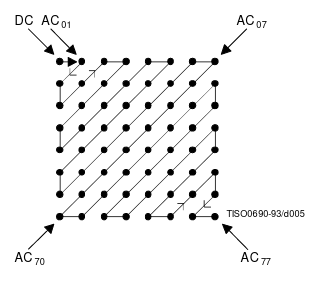
\includegraphics{zigzag.png}
    \caption{Zig-zag order}
\end{figure}

\subsection{Testing}






\newpage
\section{Results}

this section presents the results of the solutions.  It should include information on experimental settings.  The results should demonstrate the claimed benefits/disadvantages of the proposed solutions.

This section should be between 2 to 3 pages in length.
\newpage
\section{Evaluation}

This section should between 1 to 2 pages in length.
\newpage
\section{Conclusions}

This section summarises the main points of this paper.  Do not replicate the abstract as the conclusion.  A conclusion might elaborate on the importance of the work or suggest applications and extensions.  This section should be no more than 1 page in length.

The page lengths given for each section are indicative and will vary from project to project but should not exceed the upper limit.  A summary is shown in Table \ref{summary}.

\begin{table}[htb]
    \centering
    \caption{SUMMARY OF PAGE LENGTHS FOR SECTIONS}
    \vspace*{6pt}
    \label{summary}
    \begin{tabular}{|ll|c|} \hline
             & \multicolumn{1}{c|}{\bf Section} & {\bf Number of Pages} \\ \hline
        I.   & Introduction                     & 2--3                  \\ \hline
        II.  & Related Work                     & 2--3                  \\ \hline
        III. & Solution                         & 4--7                  \\ \hline
        IV.  & Results                          & 2--3                  \\ \hline
        V.   & Evaluation                       & 1-2                   \\ \hline
        VI.  & Conclusions                      & 1                     \\ \hline
    \end{tabular}
\end{table}

\newpage
\bibliography{projectpaper}


\end{document}